\section{Reinforcement Learning}
\label{sec:rl-foundations}

This section formalizes the problem of learning from interaction
and develops the algorithms used to solve it. It then shows why
these algorithms need to be extended before they can handle
high-dimensional inputs like images.

\subsection{Markov Decision Processes}
\label{subsec:mdp}

Consider the grid-world in \cref{fig:grid-world}: a player starts
in the bottom-left cell of a $3 \times 3$ grid and must reach the
top-right corner. At each step, the player chooses to move up,
down, left, or right. Most moves score zero, but reaching the goal
scores $+1$ and stepping on the center cell scores $-1$. The player
has no map and no instructions -- only the score after each move.

\begin{figure}[h!]
\centering

% Shared styles
\tikzset{
    gw cell/.style={minimum size=1.15cm, draw=black!40, thick,
                    font=\small},
    gw wall/.style={gw cell, fill=black!15},
    gw goal/.style={gw cell, fill=green!12},
    gw trap/.style={gw cell, fill=red!10},
    gw reward/.style={font=\small\bfseries},
    gw action/.style={->, thick, >=stealth, black!60,
                      shorten >=3pt, shorten <=3pt},
    gw agent/.style={circle, fill=blue!45, inner sep=4pt},
}

% Macro for the 4x3 grid skeleton
\newcommand{\gridbase}{%
    \def\s{1.15}%
    % Row 0 (bottom)
    \node[gw cell] (c00) at (0, 0) {};
    \node[gw cell] (c10) at (\s, 0) {};
    \node[gw cell] (c20) at (2*\s, 0) {};
    \node[gw cell] (c30) at (3*\s, 0) {};
    % Row 1 (middle)
    \node[gw cell] (c01) at (0, \s) {};
    \node[gw wall] (c11) at (\s, \s) {};
    \node[gw cell] (c21) at (2*\s, \s) {};
    \node[gw cell] (c31) at (3*\s, \s) {};
    % Row 2 (top)
    \node[gw cell] (c02) at (0, 2*\s) {};
    \node[gw cell] (c12) at (\s, 2*\s) {};
    \node[gw cell] (c22) at (2*\s, 2*\s) {};
    \node[gw cell] (c32) at (3*\s, 2*\s) {};
}

%% Panel (a): States -- the environment layout
\begin{subfigure}[t]{0.32\textwidth}
\centering
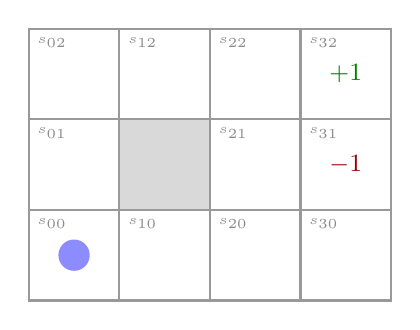
\begin{tikzpicture}
    \gridbase
    % State labels in top-left corner of each accessible cell
    \node[font=\tiny, text=black!45, anchor=north west]
          at (c00.north west) {$s_{00}$};
    \node[font=\tiny, text=black!45, anchor=north west]
          at (c10.north west) {$s_{10}$};
    \node[font=\tiny, text=black!45, anchor=north west]
          at (c20.north west) {$s_{20}$};
    \node[font=\tiny, text=black!45, anchor=north west]
          at (c30.north west) {$s_{30}$};
    \node[font=\tiny, text=black!45, anchor=north west]
          at (c01.north west) {$s_{01}$};
    % c11 is a wall -- not a state
    \node[font=\tiny, text=black!45, anchor=north west]
          at (c21.north west) {$s_{21}$};
    \node[font=\tiny, text=black!45, anchor=north west]
          at (c31.north west) {$s_{31}$};
    \node[font=\tiny, text=black!45, anchor=north west]
          at (c02.north west) {$s_{02}$};
    \node[font=\tiny, text=black!45, anchor=north west]
          at (c12.north west) {$s_{12}$};
    \node[font=\tiny, text=black!45, anchor=north west]
          at (c22.north west) {$s_{22}$};
    \node[font=\tiny, text=black!45, anchor=north west]
          at (c32.north west) {$s_{32}$};
    % Agent at start
    \node[gw agent] at (c00) {};
    % Goal and trap markers
    \node[gw reward, text=green!50!black] at (c32) {$+1$};
    \node[gw reward, text=red!60!black]   at (c31) {$-1$};
\end{tikzpicture}
\subcaption{Each cell is a \emph{state}; eleven in total.}
\label{fig:grid-world-states}
\end{subfigure}
\hfill
%% Panel (b): Actions -- movement choices
\begin{subfigure}[t]{0.32\textwidth}
\centering
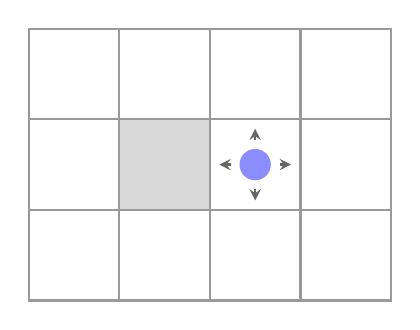
\begin{tikzpicture}
    \gridbase
    % Agent in c21 -- all four neighbors are grid cells
    \node[gw agent] (agent) at (c21) {};
    % Four action arrows to neighboring cells
    \draw[gw action] (agent.north) -- (c22.south);
    \draw[gw action] (agent.south) -- (c20.north);
    \draw[gw action] (agent.west)  -- (c11.east);
    \draw[gw action] (agent.east)  -- (c31.west);
\end{tikzpicture}
\subcaption{Moves are \emph{actions}.}
\label{fig:grid-world-actions}
\end{subfigure}
\hfill
%% Panel (c): Rewards -- feedback from the environment
\begin{subfigure}[t]{0.32\textwidth}
\centering
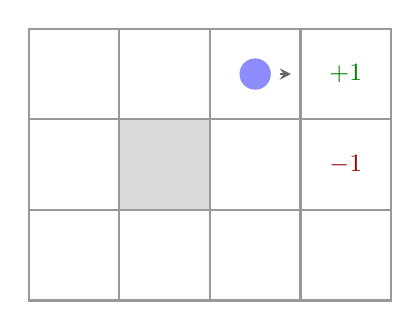
\begin{tikzpicture}
    \gridbase
    % Agent about to step into goal or trap
    \node[gw agent] (agent) at (c22) {};
    \draw[gw action] (agent.east) -- (c32.west);
    % Reward labels inside target cells
    \node[gw reward, text=green!50!black] at (c32) {$+1$};
    \node[gw reward, text=red!60!black]   at (c31) {$-1$};
\end{tikzpicture}
\subcaption{Feedback is the \emph{reward}.}
\label{fig:grid-world-rewards}
\end{subfigure}

\caption{A grid-world MDP\@. An agent (blue circle) navigates a
  $4 \times 3$ grid from a starting cell toward a goal while
  avoiding a penalty. (a)~Each accessible cell is a state, labeled
  by column and row; the shaded wall is impassable, giving eleven
  states in total. (b)~At each step the agent chooses a direction
  to move. (c)~Reaching the goal yields $+1$; the penalty
  yields~$-1$.}
\label{fig:grid-world}
\end{figure}


\smallskip
The player is the \emph{agent}, and the grid is the
\emph{environment}. At each step, the agent observes which cell it
occupies (its \emph{state}), chooses a direction to move (an
\emph{action}), and receives a score (the \emph{reward}). This
cycle repeats, and the agent's goal is to discover a strategy that
accumulates as much reward as possible over time. The \emph{Markov
decision process} (MDP)~\citep{sutton2018reinforcement} is the
mathematical framework that formalizes this cycle.

\smallskip
In the MDP notation, each step is indexed by a time step
$t = 0, 1, 2, \ldots$. The agent's current cell is $S_t$ (the
state at time~$t$), its chosen direction is $A_t$ (the action),
the score it receives is $R_{t+1}$ (the reward), and the cell it
lands in is $S_{t+1}$ (the next state). One complete cycle of these
four quantities is called a \emph{transition}:
$(S_t, A_t, R_{t+1}, S_{t+1})$.

\smallskip
When we need to refer to a specific cell rather than a time step,
we label it by its position in the grid: $s_{01}$ is the cell in
column~0, row~1 (the left-center cell). Capital~$S_t$ means ``the
state at time~$t$, whichever cell that happens to be'';
lowercase~$s_{01}$ names a fixed cell.

\smallskip
Writing $\mathcal{S}$ for the set of states and $\mathcal{A}$ for
the set of actions, the remaining piece of the MDP is the
\emph{dynamics function}~$p$. It describes what happens when the
agent acts: given state~$s$ and action~$a$, the function~$p$ gives
the probability of landing in state~$s'$ and receiving reward~$r$:
%
\begin{equation}
\label{eq:mdp-dynamics}
p(s', r \mid s, a)
  \;\doteq\;
  \Pr\{S_t = s',\, R_t = r \mid S_{t-1} = s,\, A_{t-1} = a\}.
\end{equation}
%
For any state--action pair $(s, a)$, these probabilities sum to one
over all possible next states and rewards -- exactly one outcome
must occur.

\smallskip
In our grid-world, moving right from a given cell always takes
the agent to the cell on its right -- the dynamics are
deterministic. But imagine a slippery version of the same grid:
choosing ``right'' usually moves right but occasionally slides
the agent up or down instead. The dynamics function~$p$ is a
probability distribution rather than a deterministic mapping
because it must handle this kind of uncertainty.

\smallskip
The framework rests on one key assumption, the \emph{Markov
property}: the probability of reaching any next state and reward
depends only on the current state and action, not on the history of
states and actions that came before. In the grid-world, knowing
which cell the agent is in right now is enough to determine what
happens next. It does not matter whether the agent arrived from
below, from the left, or by a longer winding path.

\smallskip
This is what makes the problem tractable. If the outcome depended
on the agent's entire history -- every state it had visited and
every action it had taken -- the agent would need to track an
ever-growing record of past experience. The Markov property says
that the current state is a sufficient summary: once we know where
the agent is now, the past is irrelevant for predicting the future.

\smallskip
\cref{fig:mdp-views} illustrates several transitions from the
grid-world: each arrow is one entry of the dynamics function, with
the action label, destination state, and reward annotation
corresponding to $a$, $s'$, and $r$.

\begin{figure}[h!]
\centering

%% Left: grid-world with a short path highlighted
\begin{subfigure}[t]{0.42\textwidth}
\centering
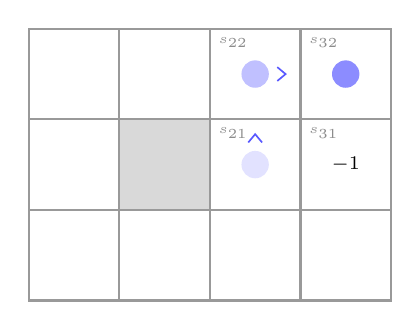
\begin{tikzpicture}[
    cell/.style={minimum size=1.15cm, draw=black!40, thick,
                 font=\scriptsize},
    wall/.style={cell, fill=black!15},
    reward/.style={font=\scriptsize\bfseries},
    agent/.style={circle, fill=blue!45, inner sep=3.5pt},
    ghost/.style={circle, fill=blue!45, inner sep=3.5pt, opacity=0.25},
    slabel/.style={font=\tiny, text=black!45},
]
\def\s{1.15}

% Row 0 (bottom)
\node[cell] (c00) at (0, 0) {};
\node[cell] (c10) at (\s, 0) {};
\node[cell] (c20) at (2*\s, 0) {};
\node[cell] (c30) at (3*\s, 0) {};
% Row 1 (middle)
\node[cell] (c01) at (0, \s) {};
\node[wall] (c11) at (\s, \s) {};
\node[cell] (c21) at (2*\s, \s) {};
\node[cell] (c31) at (3*\s, \s) {};
% Row 2 (top)
\node[cell] (c02) at (0, 2*\s) {};
\node[cell] (c12) at (\s, 2*\s) {};
\node[cell] (c22) at (2*\s, 2*\s) {};
\node[cell] (c32) at (3*\s, 2*\s) {};

% Reward labels (plain black)
\node[reward] at (c32) {$+1$};
\node[reward] at (c31) {$-1$};

% State labels in top-left corner
\node[slabel, anchor=north west] at (c21.north west) {$s_{21}$};
\node[slabel, anchor=north west] at (c22.north west) {$s_{22}$};
\node[slabel, anchor=north west] at (c32.north west) {$s_{32}$};
\node[slabel, anchor=north west] at (c31.north west) {$s_{31}$};

% Agent trail: oldest ghost most faded, recent ghost less faded,
% solid dot at current position
\node[ghost] at (c21) {};
\node[circle, fill=blue!45, inner sep=3.5pt, opacity=0.55] at (c22) {};
\node[agent] at (c32) {};

% Bare chevrons showing direction (no stem)
\draw[semithick, blue!65]
      ([yshift=8pt, xshift=-2.5pt]c21.center) --
      ([yshift=11pt]c21.center) --
      ([yshift=8pt, xshift=2.5pt]c21.center);
\draw[semithick, blue!65]
      ([xshift=8pt, yshift=2.5pt]c22.center) --
      ([xshift=11pt]c22.center) --
      ([xshift=8pt, yshift=-2.5pt]c22.center);

\end{tikzpicture}
\subcaption{Grid-world path: $s_{21} \to s_{22} \to s_{32}$.}
\label{fig:mdp-grid}
\end{subfigure}
\hfill
%% Right: same path as a state-transition graph
\begin{subfigure}[t]{0.52\textwidth}
\centering
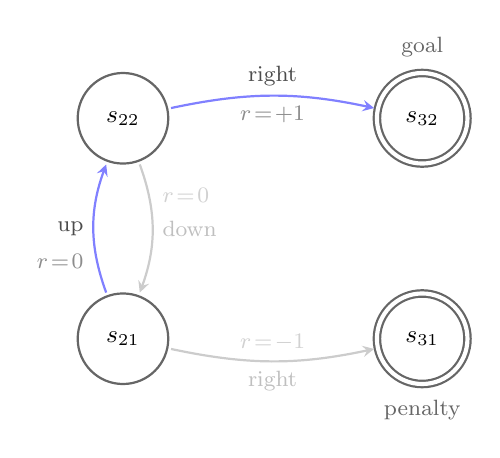
\begin{tikzpicture}[
    state/.style={circle, draw=black!60, thick,
                  minimum size=1.15cm, font=\small},
    terminal/.style={state, double, double distance=1.5pt},
    active/.style={->, thick, >=stealth, blue!50,
                   shorten >=1pt, shorten <=1pt},
    faded/.style={->, thick, >=stealth, black!20,
                  shorten >=1pt, shorten <=1pt},
    alabel/.style={font=\footnotesize, text=black!70},
    rlabel/.style={font=\footnotesize, text=black!45},
    fadea/.style={font=\footnotesize, text=black!25},
    fader/.style={font=\footnotesize, text=black!18},
]

% Nodes -- generous spacing
\node[state]    (s21) at (0, 0)     {$s_{21}$};
\node[state]    (s22) at (0, 2.8)   {$s_{22}$};
\node[terminal] (s32) at (3.8, 2.8) {$s_{32}$};
\node[terminal] (s31) at (3.8, 0)   {$s_{31}$};

% Goal/penalty annotations (plain text)
\node[font=\footnotesize, text=black!60,
      above=2pt] at (s32.north) {goal};
\node[font=\footnotesize, text=black!60,
      below=2pt] at (s31.south) {penalty};

% Active path: s21 -> s22 (up, bent left)
\draw[active] (s21) to[bend left=20]
              node[alabel, left] {up}
              node[rlabel, left, yshift=-12pt] {$r\!=\!0$}
              (s22);

% Active path: s22 -> s32 (right, bent left)
\draw[active] (s22) to[bend left=12]
              node[alabel, above] {right}
              node[rlabel, below] {$r\!=\!+1$}
              (s32);

% Faded: s22 -> s21 (down, bent left)
\draw[faded] (s22) to[bend left=20]
             node[fadea, right] {down}
             node[fader, right, yshift=12pt] {$r\!=\!0$}
             (s21);

% Faded: s21 -> s31 (right, bent right)
\draw[faded] (s21) to[bend right=12]
             node[fadea, below] {right}
             node[fader, above] {$r\!=\!-1$}
             (s31);

\end{tikzpicture}
\subcaption{The same path as a state-transition graph.}
\label{fig:mdp-graph}
\end{subfigure}

\caption{Two views of the same MDP fragment. Left: a path through
  the grid-world from $s_{21}$ to the goal. Right: the same
  states and transitions as a directed graph.}
\label{fig:mdp-views}
\end{figure}


\smallskip
The agent's goal is to collect as much reward as possible over
time -- but rewards at different times are not equally valuable.
A reward received now is worth more than the same reward received
far in the future, because the future is uncertain and because
early rewards compound. A parameter $\gamma \in [0, 1)$, called
the \emph{discount rate}, controls this trade-off. When
$\gamma = 0$, the agent cares only about the very next reward.
As $\gamma$ approaches~$1$, the agent weighs future rewards more
heavily.

\smallskip
The \emph{return} makes this precise -- it is the total discounted
reward from time step~$t$ onward:
%
\begin{equation}
\label{eq:return}
G_t \;\doteq\; R_{t+1} + \gamma\, R_{t+2} + \gamma^2 R_{t+3} + \cdots
  = \sum_{k=0}^{\infty} \gamma^k R_{t+k+1}.
\end{equation}
%
Each term $\gamma^k R_{t+k+1}$ weights a future reward by how
far away it is. Rewards received sooner count more, and very
distant rewards fade toward zero.

\smallskip
To see this concretely, suppose the agent receives rewards
$0, 0, +1$ over three steps with $\gamma = 0.9$. The return
from the first step is $G_0 = 0 + 0.9 \cdot 0 + 0.81 \cdot 1
= 0.81$ -- the distant reward of $+1$ is worth only $0.81$
today because it is discounted twice.

\smallskip
Discounting also serves a mathematical purpose: because
$\gamma < 1$, the infinite sum in \cref{eq:return} converges as
long as individual rewards are bounded. Without discounting, the
return could grow without limit.

\smallskip
\Cref{fig:discounting} illustrates the trade-off: with a low
discount rate, the agent prefers a small reward nearby over a
larger reward further away; with a high discount rate, the agent
is willing to take more steps to collect the larger reward.

\begin{figure}[h!]
\centering
% Thesis-wide categorical color palette
% Usage: % Thesis-wide categorical color palette
% Usage: \input{figures/palette} in any figure file
%
% Muted primary colors -- print-friendly, visually distinct.
% Inspired by Cooper Union's red/blue primaries, softened for
% academic figures. Use palA-palC for data series in scatter
% plots, line charts, bar charts, etc.

\definecolor{palA}{HTML}{1F77B4}   % Tableau blue
\definecolor{palB}{HTML}{D62728}   % Tableau red
\definecolor{palC}{HTML}{2CA02C}   % Tableau green
 in any figure file
%
% Muted primary colors -- print-friendly, visually distinct.
% Inspired by Cooper Union's red/blue primaries, softened for
% academic figures. Use palA-palC for data series in scatter
% plots, line charts, bar charts, etc.

\definecolor{palA}{HTML}{1F77B4}   % Tableau blue
\definecolor{palB}{HTML}{D62728}   % Tableau red
\definecolor{palC}{HTML}{2CA02C}   % Tableau green

\definecolor{agentblue}{HTML}{4C72B0}
\definecolor{rewardgreen}{HTML}{55A868}
\vspace{0.5em}

\tikzset{
    dg cell/.style={minimum size=1.0cm, draw=black!40, thick},
    dg reward/.style={font=\scriptsize\bfseries},
    dg agent/.style={circle, draw=agentblue, thick,
                     fill=agentblue!20, inner sep=2.5pt},
    dg ghost/.style={circle, draw=agentblue, thick,
                     fill=agentblue!12, inner sep=2.5pt},
    dg chev/.style={semithick, agentblue!50},
    dg slbl/.style={font=\tiny, text=black!30, anchor=north west},
    % Tree styles
    dt node/.style={circle, draw=black!40, thick,
                    minimum size=0.7cm, font=\scriptsize},
    dt start/.style={dt node, draw=agentblue, fill=agentblue!15},
    dt taken/.style={-, thick, black!45},
    dt faded/.style={-, thick, black!18, dashed},
    dt ann/.style={font=\small, text=black!60},
    dt fann/.style={font=\small, text=black!28},
    dt note/.style={font=\tiny, text=black!28},
}

%% Panel (a): Low gamma -- short path preferred
\begin{subfigure}{\textwidth}
\centering
\begin{minipage}[c]{0.32\textwidth}
\centering
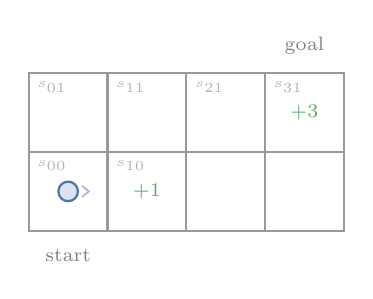
\begin{tikzpicture}
    \def\ds{1.0}
    % Row 0 (bottom)
    \node[dg cell] (g00) at (0, 0) {};
    \node[dg cell] (g10) at (\ds, 0) {};
    \node[dg cell] (g20) at (2*\ds, 0) {};
    \node[dg cell] (g30) at (3*\ds, 0) {};
    % Row 1 (top)
    \node[dg cell] (g01) at (0, \ds) {};
    \node[dg cell] (g11) at (\ds, \ds) {};
    \node[dg cell] (g21) at (2*\ds, \ds) {};
    \node[dg cell] (g31) at (3*\ds, \ds) {};
    % State labels (all path-relevant cells)
    \node[dg slbl] at (g00.north west) {$s_{00}$};
    \node[dg slbl] at (g10.north west) {$s_{10}$};
    \node[dg slbl] at (g01.north west) {$s_{01}$};
    \node[dg slbl] at (g11.north west) {$s_{11}$};
    \node[dg slbl] at (g21.north west) {$s_{21}$};
    \node[dg slbl] at (g31.north west) {$s_{31}$};
    % Rewards
    \node[dg reward, text=rewardgreen] at (g10) {$+1$};
    \node[dg reward, text=rewardgreen] at (g31) {$+3$};
    % Agent at start with right chevron (going to +1)
    \node[dg agent] at (g00) {};
    \draw[dg chev]
          ([xshift=5pt, yshift=2pt]g00.center) --
          ([xshift=7.5pt]g00.center) --
          ([xshift=5pt, yshift=-2pt]g00.center);
    % Start and goal labels
    \node[font=\scriptsize, text=black!50, below=3pt]
        at (g00.south) {start};
    \node[font=\scriptsize, text=black!50, above=3pt]
        at (g31.north) {goal};
\end{tikzpicture}
\end{minipage}%
\hfill
\begin{minipage}[c]{0.62\textwidth}
\centering
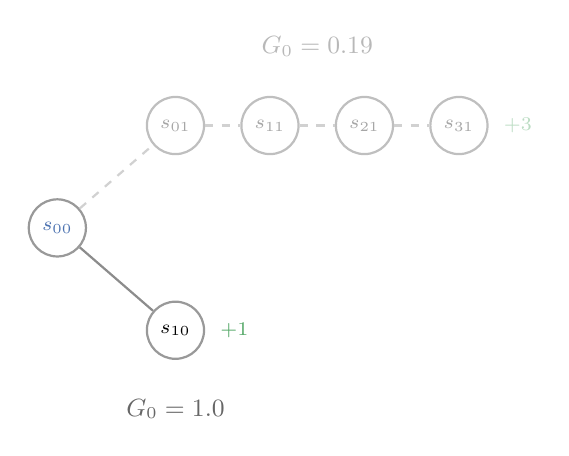
\begin{tikzpicture}
    % Start
    \node[dt node, font=\scriptsize\bfseries, text=agentblue]
        (s0) at (0, 0) {$s_{00}$};
    % Short path (taken)
    \node[dt node] (r1) at (1.5, -1.3) {$s_{10}$};
    \node[dg reward, text=rewardgreen, right=2pt] at (r1.east)
        {$+1$};
    \draw[dt taken] (s0) -- (r1);
    % Long path (faded)
    \node[dt node, draw=black!25, text=black!35] (t1) at (1.5, 1.3) {$s_{01}$};
    \node[dt node, draw=black!25, text=black!35] (t2) at (2.7, 1.3) {$s_{11}$};
    \node[dt node, draw=black!25, text=black!35] (t3) at (3.9, 1.3) {$s_{21}$};
    \node[dt node, draw=black!25, text=black!35] (r3) at (5.1, 1.3) {$s_{31}$};
    \node[dg reward, text=rewardgreen!40, right=2pt] at (r3.east)
        {$+3$};
    \draw[dt faded] (s0) -- (t1);
    \draw[dt faded] (t1) -- (t2);
    \draw[dt faded] (t2) -- (t3);
    \draw[dt faded] (t3) -- (r3);
    % Return annotations
    \node[dt ann, ] at (1.5, -2.3) {$G_0 = 1.0$};
    \node[dt fann] at (3.3, 2.3) {$G_0 = 0.19$};
\end{tikzpicture}
\end{minipage}
\vspace{0.3em}
\subcaption{$\gamma = 0.5$: the nearby $+1$ is preferred.}
\label{fig:discount-low}
\end{subfigure}

\vspace{0.6em}

%% Panel (b): High gamma -- long path preferred
\begin{subfigure}{\textwidth}
\centering
\begin{minipage}[c]{0.32\textwidth}
\centering
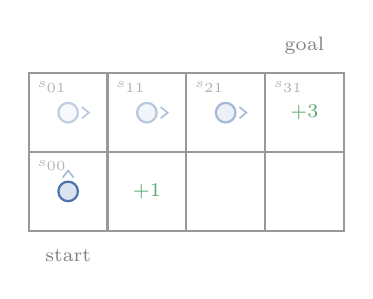
\begin{tikzpicture}
    \def\ds{1.0}
    % Row 0 (bottom)
    \node[dg cell] (g00) at (0, 0) {};
    \node[dg cell] (g10) at (\ds, 0) {};
    \node[dg cell] (g20) at (2*\ds, 0) {};
    \node[dg cell] (g30) at (3*\ds, 0) {};
    % Row 1 (top)
    \node[dg cell] (g01) at (0, \ds) {};
    \node[dg cell] (g11) at (\ds, \ds) {};
    \node[dg cell] (g21) at (2*\ds, \ds) {};
    \node[dg cell] (g31) at (3*\ds, \ds) {};
    % State labels
    \node[dg slbl] at (g00.north west) {$s_{00}$};
    \node[dg slbl] at (g01.north west) {$s_{01}$};
    \node[dg slbl] at (g11.north west) {$s_{11}$};
    \node[dg slbl] at (g21.north west) {$s_{21}$};
    \node[dg slbl] at (g31.north west) {$s_{31}$};
    % Rewards
    \node[dg reward, text=rewardgreen] at (g10) {$+1$};
    \node[dg reward, text=rewardgreen] at (g31) {$+3$};
    % Agent at start with up chevron (taking long path)
    \node[dg agent] at (g00) {};
    \draw[dg chev]
          ([yshift=5pt, xshift=-2pt]g00.center) --
          ([yshift=7.5pt]g00.center) --
          ([yshift=5pt, xshift=2pt]g00.center);
    % Ghost trail
    \node[dg ghost, draw=agentblue!35, fill=agentblue!5]
        at (g01) {};
    \node[dg ghost, draw=agentblue!40, fill=agentblue!7]
        at (g11) {};
    \node[dg ghost, draw=agentblue!50, fill=agentblue!10]
        at (g21) {};
    % Chevrons
    \draw[dg chev, agentblue!40]
          ([xshift=5pt, yshift=2pt]g01.center) --
          ([xshift=7.5pt]g01.center) --
          ([xshift=5pt, yshift=-2pt]g01.center);
    \draw[dg chev, agentblue!45]
          ([xshift=5pt, yshift=2pt]g11.center) --
          ([xshift=7.5pt]g11.center) --
          ([xshift=5pt, yshift=-2pt]g11.center);
    \draw[dg chev, agentblue!50]
          ([xshift=5pt, yshift=2pt]g21.center) --
          ([xshift=7.5pt]g21.center) --
          ([xshift=5pt, yshift=-2pt]g21.center);
    % Start and goal labels
    \node[font=\scriptsize, text=black!50, below=3pt]
        at (g00.south) {start};
    \node[font=\scriptsize, text=black!50, above=3pt]
        at (g31.north) {goal};
\end{tikzpicture}
\end{minipage}%
\hfill
\begin{minipage}[c]{0.62\textwidth}
\centering
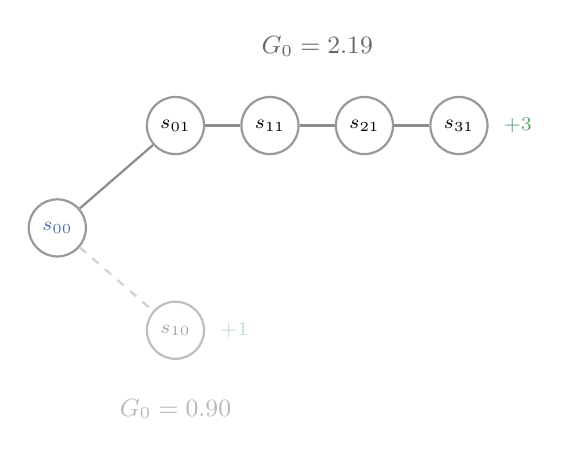
\begin{tikzpicture}
    % Start
    \node[dt node, font=\scriptsize\bfseries, text=agentblue]
        (s0) at (0, 0) {$s_{00}$};
    % Short path (faded)
    \node[dt node, draw=black!25, text=black!35] (r1) at (1.5, -1.3) {$s_{10}$};
    \node[dg reward, text=rewardgreen!40, right=2pt] at (r1.east)
        {$+1$};
    \draw[dt faded] (s0) -- (r1);
    % Long path (taken)
    \node[dt node] (t1) at (1.5, 1.3) {$s_{01}$};
    \node[dt node] (t2) at (2.7, 1.3) {$s_{11}$};
    \node[dt node] (t3) at (3.9, 1.3) {$s_{21}$};
    \node[dt node] (r3) at (5.1, 1.3) {$s_{31}$};
    \node[dg reward, text=rewardgreen, right=2pt] at (r3.east)
        {$+3$};
    \draw[dt taken] (s0) -- (t1);
    \draw[dt taken] (t1) -- (t2);
    \draw[dt taken] (t2) -- (t3);
    \draw[dt taken] (t3) -- (r3);
    % Return annotations
    \node[dt fann, ] at (1.5, -2.3) {$G_0 = 0.90$};
    \node[dt ann] at (3.3, 2.3) {$G_0 = 2.19$};
\end{tikzpicture}
\end{minipage}
\vspace{0.3em}
\subcaption{$\gamma = 0.9$: the distant $+3$ is preferred.}
\label{fig:discount-high}
\end{subfigure}

\vspace{0.5em}
\caption{The discount rate determines which path the agent prefers.
  Left: a grid with a nearby $+1$ and a distant $+3$. Right: the
  same choice as a decision tree with computed returns.}
\label{fig:discounting}
\end{figure}


\smallskip
In many problems, the interaction breaks naturally into
\emph{episodes} -- finite sequences that end in a terminal state
and then reset. The grid-world is episodic: the agent starts in
the bottom-left cell, takes a sequence of moves, and the episode ends
when it reaches the goal or the penalty. Most reinforcement
learning benchmark environments are episodic, so in practice the
return reduces to a finite sum over the steps within each episode.

\smallskip
Given an MDP, the agent needs a rule for choosing actions. This
rule is called a \emph{policy}, written $\pi(a \mid s)$, which
gives the probability of selecting action~$a$ in state~$s$. A
deterministic policy always picks the same action in a given state,
while a stochastic policy samples from a distribution over actions.

\smallskip
In the grid-world, a policy assigns a direction to each cell:
``go right when in the bottom-left cell, go up when in the cell
above it,'' and so on for every cell in the grid. A different
policy -- choosing different directions in some cells -- would
trace a different path and potentially collect different rewards.

\smallskip
The central question of reinforcement learning is how to find a
policy that maximizes the expected return -- and answering that
question requires a way to evaluate how good a given policy is,
which leads to value functions.

\subsection{Value Functions}
\label{subsec:value-functions}

A policy tells the agent what to do, but not how well it will do.
To compare policies -- and ultimately find the best one -- the
agent needs a way to assign a numerical score to each state,
capturing how much reward it can expect from that point onward.

\smallskip
But what does ``expect'' mean when outcomes are uncertain? If the
agent is in a state where going right leads to reward $+1$ with
probability $0.8$ (it reaches the goal) and reward $0$ with
probability $0.2$ (it slips and stays put), the
\emph{expected value} of that action's reward is
$0.8 \times (+1) + 0.2 \times 0 = 0.8$ -- the average outcome,
weighted by the probability of each possibility. The agent does
not actually receive $0.8$; it gets either $+1$ or $0$. But $0.8$
is the long-run average if this situation were repeated many times.
We write $\mathbb{E}[X]$ for the expected value of a random
quantity~$X$. When the expectation depends on a specific
policy~$\pi$, we write $\mathbb{E}_\pi[\cdot]$ to indicate that
the probabilities come from following that policy.

\smallskip
The \emph{state-value function} $v_\pi(s)$ answers exactly this
question: it gives the expected return when starting in state~$s$
and following policy~$\pi$ thereafter:
%
\begin{equation}
\label{eq:v-pi}
v_\pi(s) \;\doteq\; \mathbb{E}_\pi\!\big[G_t \mid S_t = s\big].
\end{equation}
%
The subscript~$\pi$ on the expectation means that the agent
follows policy~$\pi$ at every step -- the average is taken over
all the randomness in the trajectory (action choices and
transitions) that this policy produces.

\smallskip
In the grid-world, $v_\pi(s)$ is the average total reward the
agent collects from cell~$s$ onward if it follows policy~$\pi$.
Cells near the goal have high values because the agent reaches
the $+1$ reward quickly; cells near the penalty have low values
because the policy is likely to lead there.

\smallskip
\cref{fig:value-grid} makes this concrete: panel~(a) shows the
value of each cell under a policy that navigates toward the goal,
while panel~(b) shows the policy itself. The values form a
gradient -- highest near the goal, decreasing with distance.

\begin{figure}[h!]
\centering
% Thesis-wide categorical color palette
% Usage: % Thesis-wide categorical color palette
% Usage: \input{figures/palette} in any figure file
%
% Muted primary colors -- print-friendly, visually distinct.
% Inspired by Cooper Union's red/blue primaries, softened for
% academic figures. Use palA-palC for data series in scatter
% plots, line charts, bar charts, etc.

\definecolor{palA}{HTML}{1F77B4}   % Tableau blue
\definecolor{palB}{HTML}{D62728}   % Tableau red
\definecolor{palC}{HTML}{2CA02C}   % Tableau green
 in any figure file
%
% Muted primary colors -- print-friendly, visually distinct.
% Inspired by Cooper Union's red/blue primaries, softened for
% academic figures. Use palA-palC for data series in scatter
% plots, line charts, bar charts, etc.

\definecolor{palA}{HTML}{1F77B4}   % Tableau blue
\definecolor{palB}{HTML}{D62728}   % Tableau red
\definecolor{palC}{HTML}{2CA02C}   % Tableau green

\definecolor{agentblue}{HTML}{4C72B0}
\definecolor{rewardgreen}{HTML}{55A868}
\definecolor{penaltyred}{HTML}{C44E52}

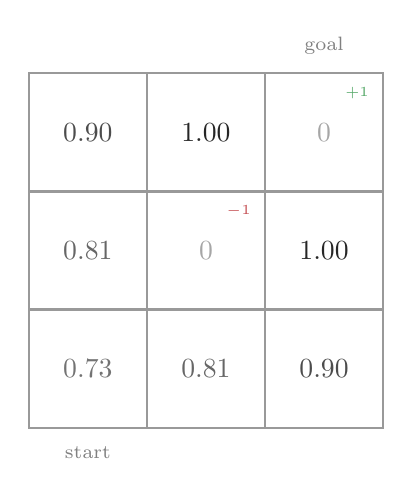
\begin{tikzpicture}[
    cell/.style={minimum size=1.5cm, draw=black!40, thick},
    val/.style={font=\normalsize},
    reward/.style={font=\normalsize\bfseries},
    agent/.style={circle, draw=agentblue, thick,
                  fill=agentblue!20, inner sep=3.5pt},
]
\def\s{1.5}

% Grid
\foreach \x in {0,1,2} {
    \foreach \y in {0,1,2} {
        \node[cell] (c\x\y) at (\x*\s, \y*\s) {};
    }
}

% Values
\node[val, text=black!55] at (c00) {0.73};
\node[val, text=black!60] at (c10) {0.81};
\node[val, text=black!70] at (c20) {0.90};
\node[val, text=black!60] at (c01) {0.81};
% s_11: penalty (terminal, v=0, reward shown in corner)
\node[val, text=black!35] at (c11) {0};
\node[font=\tiny\bfseries, text=penaltyred, anchor=north east]
    at ([xshift=-2pt, yshift=-2pt]c11.north east) {$-1$};

\node[val, text=black!85] at (c21) {1.00};
\node[val, text=black!70] at (c02) {0.90};
\node[val, text=black!85] at (c12) {1.00};

% s_22: goal (terminal, v=0, reward shown in corner)
\node[val, text=black!35] at (c22) {0};
\node[font=\tiny\bfseries, text=rewardgreen, anchor=north east]
    at ([xshift=-2pt, yshift=-2pt]c22.north east) {$+1$};


% Labels
\node[font=\scriptsize, text=black!50, below=3pt]
    at (c00.south) {start};
\node[font=\scriptsize, text=black!50, above=3pt]
    at (c22.north) {goal};

\end{tikzpicture}

\vspace{0.5em}
\caption{State values $v_\pi(s)$ in the grid-world ($\gamma = 0.9$).
  Values increase with proximity to the goal; terminal cells have
  $v = 0$ (corner labels show the entry reward).}
\label{fig:value-grid}
\end{figure}


\smallskip
The state-value function tells us how good a state is, but it
does not tell us which action to take. For that, we need the
\emph{action-value function} $q_\pi(s, a)$, which gives the
expected return for taking action~$a$ in state~$s$ and then
following~$\pi$:
%
\begin{equation}
\label{eq:q-pi}
q_\pi(s, a) \;\doteq\; \mathbb{E}_\pi\!\big[G_t \mid S_t = s,\, A_t = a\big].
\end{equation}
%
The difference is subtle but important: $v_\pi$ evaluates
\emph{states}, while $q_\pi$ evaluates \emph{actions in states}.

\smallskip
In the grid-world, consider the agent in cell~$s_{21}$.
Moving up leads toward the $+1$ goal, so
$q_\pi(s_{21}, \text{up})$ is high. Moving right leads directly
to the $-1$ penalty in $s_{31}$, so
$q_\pi(s_{21}, \text{right})$ is low. The state value $v_\pi$
assigns a single number to~$s_{21}$, but the action values reveal
that the actions available there are dramatically different.
\Cref{fig:q-values} shows this: each arrow from~$s_{21}$ carries
a different Q-value, making the best action immediately apparent.

\begin{figure}[ht]
\centering
% Thesis-wide categorical color palette
% Usage: % Thesis-wide categorical color palette
% Usage: \input{figures/palette} in any figure file
%
% Muted primary colors -- print-friendly, visually distinct.
% Inspired by Cooper Union's red/blue primaries, softened for
% academic figures. Use palA-palC for data series in scatter
% plots, line charts, bar charts, etc.

\definecolor{palA}{HTML}{1F77B4}   % Tableau blue
\definecolor{palB}{HTML}{D62728}   % Tableau red
\definecolor{palC}{HTML}{2CA02C}   % Tableau green
 in any figure file
%
% Muted primary colors -- print-friendly, visually distinct.
% Inspired by Cooper Union's red/blue primaries, softened for
% academic figures. Use palA-palC for data series in scatter
% plots, line charts, bar charts, etc.

\definecolor{palA}{HTML}{1F77B4}   % Tableau blue
\definecolor{palB}{HTML}{D62728}   % Tableau red
\definecolor{palC}{HTML}{2CA02C}   % Tableau green

\definecolor{agentblue}{HTML}{4C72B0}
\definecolor{rewardgreen}{HTML}{55A868}
\definecolor{penaltyred}{HTML}{C44E52}

%% Left: grid showing s_21
\begin{subfigure}[b]{0.32\textwidth}
\centering
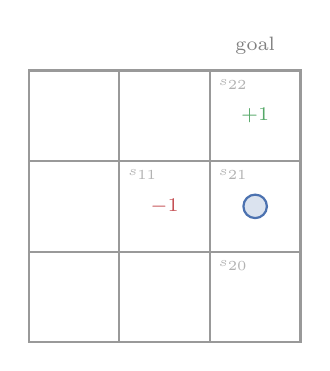
\begin{tikzpicture}[
    cell/.style={minimum size=1.15cm, draw=black!40, thick},
    reward/.style={font=\scriptsize\bfseries},
    agent/.style={circle, draw=agentblue, thick,
                  fill=agentblue!20, inner sep=3pt},
    slbl/.style={font=\tiny, text=black!30, anchor=north west},
]
\def\s{1.15}

% Grid
\foreach \x in {0,1,2} {
    \foreach \y in {0,1,2} {
        \node[cell] (c\x\y) at (\x*\s, \y*\s) {};
    }
}

% Rewards
\node[reward, text=rewardgreen] at (c22) {$+1$};
\node[reward, text=penaltyred] at (c11) {$-1$};

% Labels
\node[slbl] at (c21.north west) {$s_{21}$};
\node[slbl] at (c22.north west) {$s_{22}$};
\node[slbl] at (c11.north west) {$s_{11}$};
\node[slbl] at (c20.north west) {$s_{20}$};

% Agent at s_21
\node[agent] at (c21) {};

% Goal
\node[font=\scriptsize, text=black!50, above=2pt]
    at (c22.north) {goal};

\end{tikzpicture}
\vspace{0.8em}
\subcaption{Agent in $s_{21}$.}
\label{fig:q-grid}
\end{subfigure}
\hfill
%% Right: Q-values from s_21 (star layout)
\begin{subfigure}[b]{0.62\textwidth}
\centering
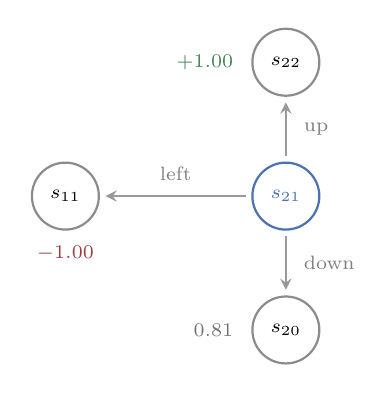
\begin{tikzpicture}[
    state/.style={circle, draw=black!45, thick,
                  minimum size=0.85cm, font=\scriptsize},
    center/.style={state, draw=agentblue,
                   font=\scriptsize\bfseries, text=agentblue},
    arr/.style={->, thick, >=stealth, black!40,
                shorten >=2pt, shorten <=2pt},
    qlbl/.style={font=\scriptsize},
    dirlbl/.style={font=\scriptsize, text=black!50},
]

% Center state
\node[center] (s21) at (0, 0) {$s_{21}$};

% Up -> s_22 (goal, Q = +1.00)
\node[state] (s22) at (0, 1.7) {$s_{22}$};
\draw[arr] (s21) -- (s22);
\node[dirlbl, right=3pt] at (0, 0.85) {up};
\node[qlbl, text=rewardgreen!80!black, left=3pt]
    at (s22.west) {$+1.00$};

% Left -> s_11 (penalty, Q = -1.00)
\node[state] (s11) at (-2.8, 0) {$s_{11}$};
\draw[arr] (s21) -- (s11);
\node[dirlbl, above=2pt] at (-1.4, 0) {left};
\node[qlbl, text=penaltyred!80!black, below=2pt]
    at (s11.south) {$-1.00$};

% Down -> s_20 (Q = 0.81)
\node[state] (s20) at (0, -1.7) {$s_{20}$};
\draw[arr] (s21) -- (s20);
\node[dirlbl, right=3pt] at (0, -0.85) {down};
\node[qlbl, text=black!55, left=3pt]
    at (s20.west) {$0.81$};

\end{tikzpicture}
\vspace{0.8em}
\subcaption{Q-values: same state, different actions.}
\label{fig:q-values-star}
\end{subfigure}

\vspace{0.5em}
\caption{Action values $q_\pi(s_{21}, a)$. From the same state,
  different actions have dramatically different values.}
\label{fig:q-values}
\end{figure}


\smallskip
This is why $q_\pi$ is more directly useful for decision-making
than $v_\pi$: comparing Q-values across actions tells the agent
which action to take, without needing a model of the environment.

\smallskip
Both value functions are defined as expectations over the entire
future -- averages over every possible trajectory from the current
state onward. Computing them from these definitions directly would
require enumerating all such trajectories, which quickly becomes
impractical. The next section shows that the Markov property provides
a recursive shortcut.

\subsection{The Bellman Equation}
\label{subsec:bellman-equation}

Computing $v_\pi$ from its definition means averaging the return over
every possible trajectory from state~$s$ -- every sequence of
actions, transitions, and rewards stretching to the end of the
episode. Even for the grid-world, the number of trajectories grows
exponentially with the episode length. For larger problems, this
direct approach is hopeless.

\smallskip
The Markov property from \cref{subsec:mdp} provides a way out.
Because the future depends only on the current state, the value of a
state can be decomposed into two pieces: the reward from the next
step, and the discounted value of wherever the agent ends up. For
$v_\pi$, this gives the \emph{Bellman expectation equation}:
%
\begin{equation}
\label{eq:bellman-expectation}
v_\pi(s) = \sum_{a} \pi(a \mid s) \sum_{s',\, r}
  p(s', r \mid s, a)\,\big[r + \gamma\, v_\pi(s')\big].
\end{equation}
%
In words: the value of state~$s$ is the average, over all actions the
policy might take, of the immediate reward plus the discounted value
of the next state.

\smallskip
The equation has three layers, each handling a different source of
uncertainty. The outer sum weights actions by $\pi(a \mid s)$ -- the
probability the policy assigns to each action. The inner sum weights
outcomes by $p(s', r \mid s, a)$ -- the environment's transition
probabilities. And the bracketed term $r + \gamma\, v_\pi(s')$ is the
one-step payoff: the reward received now, plus the discounted value of
the successor state. \cref{fig:bellman-backup} shows this structure
as a tree: from state~$s$, the policy selects an action, the
environment responds with a reward and next state, and the payoff at
each leaf is the immediate reward plus the discounted future value.

\begin{figure}[h!]
\centering
% Thesis-wide categorical color palette
% Usage: % Thesis-wide categorical color palette
% Usage: \input{figures/palette} in any figure file
%
% Muted primary colors -- print-friendly, visually distinct.
% Inspired by Cooper Union's red/blue primaries, softened for
% academic figures. Use palA-palC for data series in scatter
% plots, line charts, bar charts, etc.

\definecolor{palA}{HTML}{1F77B4}   % Tableau blue
\definecolor{palB}{HTML}{D62728}   % Tableau red
\definecolor{palC}{HTML}{2CA02C}   % Tableau green
 in any figure file
%
% Muted primary colors -- print-friendly, visually distinct.
% Inspired by Cooper Union's red/blue primaries, softened for
% academic figures. Use palA-palC for data series in scatter
% plots, line charts, bar charts, etc.

\definecolor{palA}{HTML}{1F77B4}   % Tableau blue
\definecolor{palB}{HTML}{D62728}   % Tableau red
\definecolor{palC}{HTML}{2CA02C}   % Tableau green

\begin{tikzpicture}[
    snode/.style={circle, draw=black!50, thick, fill=palA!12,
                  minimum size=0.9cm, font=\small},
    anode/.style={circle, fill=black!60, minimum size=5pt,
                  inner sep=0pt},
    edge/.style={thick, black!45, -Stealth},
    elabel/.style={font=\scriptsize, text=black!55},
    payoff/.style={font=\scriptsize, text=black!45},
]

% Root state
\node[snode] (s) at (0, 0) {$s$};

% Action nodes
\node[anode] (a1) at (-1.8, -1.5) {};
\node[anode] (a2) at ( 1.8, -1.5) {};
\node[font=\scriptsize, left=3pt] at (a1) {$a_1$};
\node[font=\scriptsize, right=3pt] at (a2) {$a_2$};

% Next-state nodes
\node[snode] (s1) at (-1.8, -3.4) {$s'$};
\node[snode] (s2) at ( 1.8, -3.4) {$s''$};

% Policy edges (state -> actions)
\draw[edge] (s) -- node[elabel, left, pos=0.4]
    {$\pi(a_1 \!\mid\! s)$} (a1);
\draw[edge] (s) -- node[elabel, right, pos=0.4]
    {$\pi(a_2 \!\mid\! s)$} (a2);

% Transition edges (actions -> next states)
\draw[edge] (a1) -- node[elabel, left] {$r_1$} (s1);
\draw[edge] (a2) -- node[elabel, right] {$r_2$} (s2);

% Payoff annotations
\node[payoff, below=5pt] at (s1)
    {$r_1 + \gamma\, v_\pi(s')$};
\node[payoff, below=5pt] at (s2)
    {$r_2 + \gamma\, v_\pi(s'')$};

\end{tikzpicture}
\vspace{0.5em}
\caption{Bellman backup: $v_\pi(s)$ decomposes into one step of
  reward plus the discounted value of the successor state.}
\label{fig:bellman-backup}
\end{figure}


\smallskip
To see this concretely, consider cell~$s_{21}$ in the grid-world.
Suppose the policy says ``go up'' with certainty, and moving up from
$s_{21}$ always leads to $s_{22}$ with reward $r = 0$ (the transition
is deterministic). Then both sums collapse to a single term:
%
\[
v_\pi(s_{21}) = 0 + 0.9 \times v_\pi(s_{22}).
\]
%
If $v_\pi(s_{22}) = 1.0$, then $v_\pi(s_{21}) = 0.90$ -- matching
the values shown in \cref{fig:value-grid}. The value of~$s_{21}$ is
entirely determined by the value of its neighbor; no need to trace the
trajectory all the way to the goal.

\smallskip
When the policy is stochastic -- assigning positive probability to
more than one action -- the value becomes a weighted average across
all possible actions, each weighted by the probability the policy
assigns to it. And when transitions are stochastic, there is an
additional average over the possible next states the environment might
produce. The equation handles both cases through its nested sums.

\smallskip
This equation might seem circular -- the value of a state is defined
in terms of the values of other states, which are themselves defined
the same way. But it is not circular; it is recursive. The chain of
dependencies terminates at terminal states, where the value is zero
because the episode is over and no more reward can be collected. From
there, values propagate backward: the cell next to the goal derives
its value from the goal, the cell two steps away derives its value
from the cell one step away, and so on through the grid.

\smallskip
The power of the Bellman equation is that it reduces a calculation
over the entire future -- the sum of all discounted rewards along
every possible trajectory -- to a one-step relationship between
neighboring states. Instead of tracing every path to the end of the
episode, we only need to look one step ahead. This recursion is what
makes reinforcement learning computationally tractable.

\subsection{Optimal Policies}
\label{subsec:optimal-policies}

The Bellman equation tells us how to evaluate any given policy -- but
the agent does not just want to evaluate its current strategy. It
wants to find the best one.

\smallskip
A policy $\pi^*$ is \emph{optimal} if its expected return is at least
as high as that of every other policy, in every state:
$v_{\pi^*}(s) \geq v_\pi(s)$ for all states~$s$ and all
policies~$\pi$~\citep{sutton2018reinforcement}. At least one optimal
policy always exists.

\smallskip
There may be several optimal policies -- for instance, two paths
through the grid-world might yield the same total reward. But all
optimal policies share the same value functions, which we denote
$v_*$ and $q_*$:
%
\begin{align}
\label{eq:v-star}
v_*(s) &\;\doteq\; \max_\pi\, v_\pi(s), \\[4pt]
\label{eq:q-star}
q_*(s, a) &\;\doteq\; \max_\pi\, q_\pi(s, a).
\end{align}
%
In words, $v_*(s)$ is the highest value achievable in state~$s$ under
any policy, and $q_*(s, a)$ is the highest value achievable by taking
action~$a$ in state~$s$ and then acting optimally thereafter.

\smallskip
The optimal value functions satisfy their own recursive relationship,
the \emph{Bellman optimality equation}. For $q_*$:
%
\begin{equation}
\label{eq:bellman-optimality-q}
q_*(s, a) = \sum_{s',\, r} p(s', r \mid s, a)
  \Big[r + \gamma \max_{a'} q_*(s', a')\Big].
\end{equation}
%
The key difference from the Bellman expectation equation
(\cref{eq:bellman-expectation}) is that the average over the policy's
action choices is replaced by a maximum: instead of asking ``what
return does the current policy achieve,'' we ask ``what is the best
possible return if we act optimally from here.''

\smallskip
If $q_*$ were known, acting optimally would be trivial: in every
state, the agent simply picks the action with the highest $q$-value,
$\pi^*(s) = \arg\max_a q_*(s, a)$. No model of the environment is
needed and no planning is required -- the optimal action is a direct
lookup. This is why much of reinforcement learning, including the
Q-learning algorithm in the next section and the deep Q-networks that
build on it, focuses on estimating $q_*$ rather than $v_*$.

\smallskip
There is a catch, however. The Bellman optimality equation is a
system of $|\mathcal{S}| \times |\mathcal{A}|$ simultaneous
equations, one for every state--action pair. Solving it requires
knowing the dynamics~$p$ and enumerating every state -- both of which
are impractical for any problem with a large state space or unknown
dynamics. The next two sections address these obstacles: Q-learning
estimates $q_*$ from experience without knowing the dynamics, and
function approximation replaces the explicit table of $q$-values with
a neural network that can generalize across states.

\subsection{Q-Learning}
\label{subsec:q-learning}

The Bellman optimality equation tells us what $q_*$ must satisfy,
but solving it requires knowing the dynamics~$p$. In most problems
of interest, the agent does not have this information -- it cannot
look up what will happen; it can only try an action and observe the
result. Q-learning~\citep{watkins1992q} addresses exactly this
setting: the agent learns $q_*$ directly from experience, one
transition at a time, without ever knowing $p$.

\smallskip
The key idea comes from \emph{temporal-difference} (TD)
learning~\citep{sutton1988learning}: rather than waiting until
the end of an episode to see how things turned out, the agent
updates its estimate after every single step. It observes the
immediate reward, peeks at its current estimate of the next
state's value, and uses these together as a learning target.
This peeking is called \emph{bootstrapping} -- the agent learns
from its own estimates rather than from complete outcomes. The
estimates may be wrong at first, but because each update
incorporates a real observed reward, the errors shrink over time.

\smallskip
The Q-learning update rule puts this idea into practice. After
the agent takes action~$A_t$ in state~$S_t$, observes
reward~$R_{t+1}$, and arrives in state~$S_{t+1}$, it updates
its estimate of $q_*(S_t, A_t)$:
%
\begin{equation}
\label{eq:q-learning}
Q(S_t, A_t) \;\leftarrow\; Q(S_t, A_t)
  + \alpha \Big[R_{t+1} + \gamma \max_{a} Q(S_{t+1}, a)
  - Q(S_t, A_t)\Big].
\end{equation}
%
$Q(S_t, A_t)$ is the agent's current estimate for this
state--action pair. The expression
$R_{t+1} + \gamma \max_a Q(S_{t+1}, a)$ is the \emph{TD
target} -- the reward the agent actually received, plus its best
estimate of the value from the next state onward. The difference
between the target and the current estimate is the \emph{TD
error}: how far off the agent's prediction was. The learning rate
$\alpha \in (0, 1]$ controls how far the estimate moves toward
the target on each step -- large $\alpha$ moves quickly but may
overshoot; small $\alpha$ is more stable but learns slowly.

\smallskip
To see this in the grid-world, suppose the agent is in
cell~$s_{21}$ and moves up, receiving reward $r = 0$ and
arriving in cell~$s_{22}$. If the agent currently estimates
$Q(s_{21}, \text{up}) = 0.5$ and $\max_a Q(s_{22}, a) = 1.0$,
then with $\gamma = 0.9$ and $\alpha = 0.1$:
%
\begin{align*}
\text{target} &= 0 + 0.9 \times 1.0 = 0.9, \\
\text{TD error} &= 0.9 - 0.5 = 0.4, \\
Q(s_{21}, \text{up}) &\leftarrow 0.5 + 0.1 \times 0.4 = 0.54.
\end{align*}
%
The estimate moved from $0.5$ toward the target of $0.9$ -- not
all the way, but a step in the right direction.
\Cref{fig:td-update} shows this update spatially: the value
estimate at $s_{22}$ bootstraps back to refine the estimate at
$s_{21}$. After many such updates across many transitions, the
estimates converge to $q_*$.

\begin{figure}[ht]
\centering
% Thesis-wide categorical color palette
% Usage: % Thesis-wide categorical color palette
% Usage: \input{figures/palette} in any figure file
%
% Muted primary colors -- print-friendly, visually distinct.
% Inspired by Cooper Union's red/blue primaries, softened for
% academic figures. Use palA-palC for data series in scatter
% plots, line charts, bar charts, etc.

\definecolor{palA}{HTML}{1F77B4}   % Tableau blue
\definecolor{palB}{HTML}{D62728}   % Tableau red
\definecolor{palC}{HTML}{2CA02C}   % Tableau green
 in any figure file
%
% Muted primary colors -- print-friendly, visually distinct.
% Inspired by Cooper Union's red/blue primaries, softened for
% academic figures. Use palA-palC for data series in scatter
% plots, line charts, bar charts, etc.

\definecolor{palA}{HTML}{1F77B4}   % Tableau blue
\definecolor{palB}{HTML}{D62728}   % Tableau red
\definecolor{palC}{HTML}{2CA02C}   % Tableau green


%% Panel (a): The transition on the grid
\begin{subfigure}[t]{0.42\textwidth}
\centering
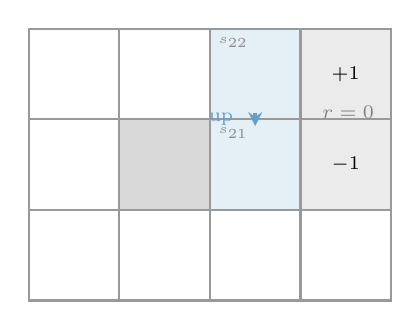
\begin{tikzpicture}[
    cell/.style={minimum size=1.15cm, draw=black!40, thick},
    wall/.style={cell, fill=black!15},
    terminal/.style={cell, fill=black!8},
    highlight/.style={cell, fill=palA!12},
    arr/.style={->, thick, >=stealth},
    plabel/.style={font=\scriptsize\bfseries},
    slabel/.style={font=\tiny, text=black!45, anchor=north west},
]
\def\s{1.15}

% Full 4x3 grid
% Row 0
\node[cell] (c00) at (0, 0) {};
\node[cell] (c10) at (\s, 0) {};
\node[cell] (c20) at (2*\s, 0) {};
\node[cell] (c30) at (3*\s, 0) {};
% Row 1
\node[cell] (c01) at (0, \s) {};
\node[wall] (c11) at (\s, \s) {};
\node[highlight] (c21) at (2*\s, \s) {};
\node[terminal] (c31) at (3*\s, \s) {};
% Row 2
\node[cell] (c02) at (0, 2*\s) {};
\node[cell] (c12) at (\s, 2*\s) {};
\node[highlight] (c22) at (2*\s, 2*\s) {};
\node[terminal] (c32) at (3*\s, 2*\s) {};

% State labels
\node[slabel] at (c21.north west) {$s_{21}$};
\node[slabel] at (c22.north west) {$s_{22}$};

% Terminal labels
\node[plabel] at (c31) {$-1$};
\node[plabel] at (c32) {$+1$};

% Action arrow
\draw[arr, palA!70, very thick]
    ([yshift=2pt]c21.north) -- ([yshift=-2pt]c22.south)
    node[midway, left=4pt, font=\scriptsize, text=palA!70]
    {up};

% Reward annotation
\node[font=\scriptsize, text=black!50, right=4pt]
    at ([yshift=2pt]c21.north east) {$r = 0$};

\end{tikzpicture}
\subcaption{The agent in $s_{21}$ moves up to $s_{22}$,
  receiving reward $r = 0$.}
\label{fig:td-update-transition}
\end{subfigure}
\hfill
%% Panel (b): The bootstrap update
\begin{subfigure}[t]{0.52\textwidth}
\centering
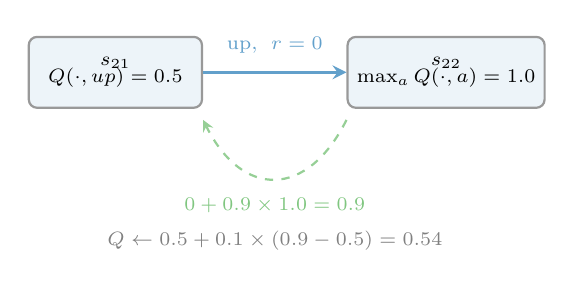
\begin{tikzpicture}[
    state/.style={draw=black!40, thick, rounded corners=3pt,
                  minimum width=2.2cm, minimum height=0.9cm,
                  font=\scriptsize, align=center, fill=palA!8},
    arr/.style={->, thick, >=stealth},
    lbl/.style={font=\scriptsize, text=black!55},
]

% State boxes (horizontal layout)
\node[state] (s21) at (0, 0)
    {$s_{21}$\\[-2pt] $Q(\cdot, \text{up}) = 0.5$};

\node[state] (s22) at (4.2, 0)
    {$s_{22}$\\[-2pt] $\max_a Q(\cdot, a) = 1.0$};

% Forward arrow: action + reward
\draw[arr, palA!70, very thick]
    (s21.east) -- (s22.west)
    node[midway, above=3pt, font=\scriptsize, text=palA!70]
    {up,\; $r = 0$};

% Bootstrap arrow (curved, below)
\draw[arr, palC!50, dashed, thick]
    ([yshift=-4pt]s22.south west)
    .. controls +(-0.5, -1.0) and +(0.5, -1.0) ..
    ([yshift=-4pt]s21.south east)
    node[midway, below=3pt, font=\scriptsize, text=palC!60]
    {$0 + 0.9 \times 1.0 = 0.9$}
    node[midway, below=15pt, font=\scriptsize, text=black!50]
    {$Q \leftarrow 0.5 + 0.1 \times (0.9 - 0.5) = 0.54$};

\end{tikzpicture}
\subcaption{The estimate at $s_{22}$ bootstraps back.
  The target updates $Q(s_{21}, \text{up})$ toward $0.9$.}
\label{fig:td-update-bootstrap}
\end{subfigure}

\caption{One Q-learning update step in the grid-world.}
\label{fig:td-update}
\end{figure}


\smallskip
The connection to the Bellman optimality equation
(\cref{eq:bellman-optimality-q}) is direct: the TD target
$R_{t+1} + \gamma \max_a Q(S_{t+1}, a)$ is a single-sample
estimate of the right-hand side of that equation. Each update
nudges the Q-values toward satisfying the Bellman optimality
equation, using real experience instead of known dynamics.

\smallskip
There is a tension, however, between learning and acting. If the
agent always picks the action with the highest Q-value -- the
\emph{greedy} action -- it will exploit what it currently knows
but may never discover that a different action is better. In the
grid-world, an agent that found a path to the $+1$ reward early
on might follow it forever, never exploring the route that leads
to a higher reward elsewhere. \cref{fig:exploration} shows this
tension in miniature: a greedy agent stays with the known $+1$
and never discovers the $+3$.

\begin{figure}[h!]
\centering
% Thesis-wide categorical color palette
% Usage: % Thesis-wide categorical color palette
% Usage: \input{figures/palette} in any figure file
%
% Muted primary colors -- print-friendly, visually distinct.
% Inspired by Cooper Union's red/blue primaries, softened for
% academic figures. Use palA-palC for data series in scatter
% plots, line charts, bar charts, etc.

\definecolor{palA}{HTML}{1F77B4}   % Tableau blue
\definecolor{palB}{HTML}{D62728}   % Tableau red
\definecolor{palC}{HTML}{2CA02C}   % Tableau green
 in any figure file
%
% Muted primary colors -- print-friendly, visually distinct.
% Inspired by Cooper Union's red/blue primaries, softened for
% academic figures. Use palA-palC for data series in scatter
% plots, line charts, bar charts, etc.

\definecolor{palA}{HTML}{1F77B4}   % Tableau blue
\definecolor{palB}{HTML}{D62728}   % Tableau red
\definecolor{palC}{HTML}{2CA02C}   % Tableau green


%% Panel (a): Pure exploitation
\begin{subfigure}[t]{0.45\textwidth}
\centering
\begin{tikzpicture}[
    snode/.style={circle, draw=black!50, thick, fill=palA!12,
                  minimum size=0.9cm, font=\small},
    rnode/.style={circle, draw=black!40, thick,
                  minimum size=0.9cm, font=\small\bfseries},
    chosen/.style={very thick, palA, -Stealth},
    unchosen/.style={thick, black!25, dashed, -Stealth},
    qlabel/.style={font=\scriptsize},
]

\node[snode] (s) at (0, 0) {$s$};
\node[rnode, fill=palA!8] (r1) at (-1.6, -2) {$+1$};
\node[rnode, fill=black!5] (r2) at ( 1.6, -2) {?};

\draw[chosen] (s) -- node[qlabel, left, pos=0.4]
    {$Q\!=\!1$} (r1);
\draw[unchosen] (s) -- node[qlabel, right, pos=0.4,
    text=black!35] {$Q\!=\!0$} (r2);

\end{tikzpicture}
\vspace{0.5em}
\subcaption{Greedy: always picks the known $+1$.}
\label{fig:exploration-greedy}
\end{subfigure}
\hfill
%% Panel (b): After exploration
\begin{subfigure}[t]{0.45\textwidth}
\centering
\begin{tikzpicture}[
    snode/.style={circle, draw=black!50, thick, fill=palA!12,
                  minimum size=0.9cm, font=\small},
    rnode/.style={circle, draw=black!40, thick,
                  minimum size=0.9cm, font=\small\bfseries},
    chosen/.style={very thick, palC, -Stealth},
    unchosen/.style={thick, black!25, -Stealth},
    qlabel/.style={font=\scriptsize},
]

\node[snode] (s) at (0, 0) {$s$};
\node[rnode, fill=black!5] (r1) at (-1.6, -2) {$+1$};
\node[rnode, fill=palC!10] (r2) at ( 1.6, -2) {$+3$};

\draw[unchosen] (s) -- node[qlabel, left, pos=0.4,
    text=black!45] {$Q\!=\!1$} (r1);
\draw[chosen] (s) -- node[qlabel, right, pos=0.4]
    {$Q\!=\!3$} (r2);

\end{tikzpicture}
\vspace{0.5em}
\subcaption{Exploring discovers the $+3$ reward.}
\label{fig:exploration-discovered}
\end{subfigure}

\vspace{0.8em}
\caption{Without exploration, the agent settles for the first
  rewarding action it finds and never discovers better alternatives.}
\label{fig:exploration}
\end{figure}


\smallskip
This is the \emph{exploration--exploitation} trade-off: the agent
must sometimes try actions that look suboptimal in order to gather
information that could improve its long-term behavior. The
simplest solution is the $\epsilon$\emph{-greedy} strategy: with
probability $1 - \epsilon$ the agent takes the greedy action, and
with probability~$\epsilon$ it picks a random action instead.
Early in training, $\epsilon$ is large so the agent explores
broadly; over time, $\epsilon$ is decayed toward a small value so
the agent increasingly exploits its learned Q-values.

\smallskip
A notable property of Q-learning is that it is \emph{off-policy}:
the update rule always uses $\max_a Q(S_{t+1}, a)$ -- the value
of the best action -- regardless of which action the agent
actually takes next. The agent explores with $\epsilon$-greedy,
but the update targets the greedy (optimal) policy. This
separation is what makes exploration safe: the agent can try
random actions to discover new information without corrupting its
estimate of $q_*$.

\smallskip
Under standard conditions -- all state--action pairs continue to
be visited, and the learning rate is decreased
appropriately -- Q-learning converges to $q_*$ with probability
one~\citep{watkins1992q}. The $\epsilon$-greedy policy ensures
the visitation condition as long as $\epsilon > 0$.

\smallskip
The algorithm as described maintains a table with one entry for
every state--action pair. For the grid-world, this table has
$11 \times 4 = 44$ entries -- perfectly manageable. But for
problems with large state spaces, the table becomes impractical.
If the state is a raw image, the number of possible states grows
astronomically, and the agent would need to visit each one
repeatedly to learn its Q-values. Worse, learning that one state
is valuable tells the agent nothing about similar states it has
not yet seen -- there is no generalization.

\smallskip
The next section addresses this limitation by replacing the table
with a parameterized function that can generalize across states,
allowing Q-learning to scale to problems where explicit
enumeration is impossible.

\subsection{Function Approximation}
\label{subsec:func-approx}

Q-learning as described in the previous section maintains a table
with one entry for every state--action pair. When the state is a
raw image -- say, $84 \times 84$ grayscale pixels -- the number of
possible states is astronomical. A table cannot fit in memory, the
agent cannot visit every entry, and learning that one state is
valuable tells it nothing about similar states it has not yet seen.
Tabular Q-learning is not merely slow in such settings; it is
impossible.

\smallskip
The solution is to replace the table with a parameterized function.
Instead of storing a separate value for each state--action pair, we
define a function $Q(s, a;\, \mathbf{w})$ that takes a state and
action as input and produces a Q-value estimate as output, where
$\mathbf{w}$ is a vector of adjustable parameters (weights).

\smallskip
The key advantage is generalization. Because the function maps
states to Q-values through shared parameters, updating
$\mathbf{w}$ based on one state automatically changes the estimates
for similar states. In the grid-world analogy, this is like learning
the rule ``cells closer to the goal are worth more'' rather than
memorizing the value of each cell individually -- the rule applies
even to cells the agent has never visited.
\Cref{fig:table-vs-network} contrasts the two approaches.

\begin{figure}[ht]
\centering
% Thesis-wide categorical color palette
% Usage: % Thesis-wide categorical color palette
% Usage: \input{figures/palette} in any figure file
%
% Muted primary colors -- print-friendly, visually distinct.
% Inspired by Cooper Union's red/blue primaries, softened for
% academic figures. Use palA-palC for data series in scatter
% plots, line charts, bar charts, etc.

\definecolor{palA}{HTML}{1F77B4}   % Tableau blue
\definecolor{palB}{HTML}{D62728}   % Tableau red
\definecolor{palC}{HTML}{2CA02C}   % Tableau green
 in any figure file
%
% Muted primary colors -- print-friendly, visually distinct.
% Inspired by Cooper Union's red/blue primaries, softened for
% academic figures. Use palA-palC for data series in scatter
% plots, line charts, bar charts, etc.

\definecolor{palA}{HTML}{1F77B4}   % Tableau blue
\definecolor{palB}{HTML}{D62728}   % Tableau red
\definecolor{palC}{HTML}{2CA02C}   % Tableau green

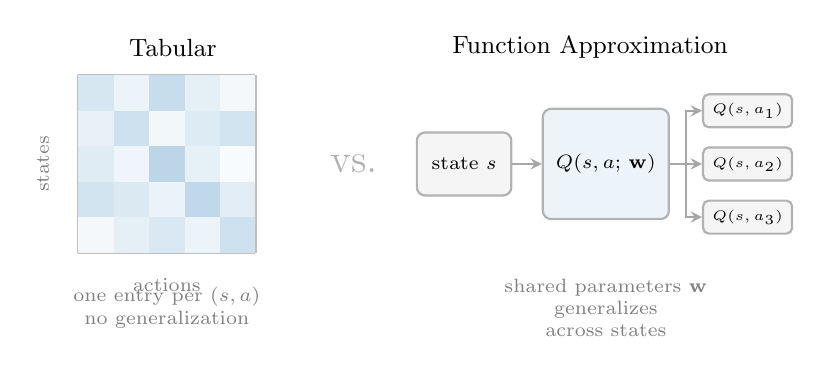
\begin{tikzpicture}[
    arr/.style={->, thick, >=stealth, black!35},
    lbl/.style={font=\small},
    sublbl/.style={font=\scriptsize, text=black!50},
]

% --- Tabular (left) ---
\node[lbl] at (1.2, 2.6) {Tabular};

% Q-table grid
\draw[thick, black!25] (0, 0) grid[step=0.45] (2.25, 2.25);

% Row/column labels
\node[sublbl, rotate=90, anchor=south] at (-0.25, 1.125) {states};
\node[sublbl, anchor=north] at (1.125, -0.2) {actions};

% Fill a few cells to suggest values
\foreach \x/\y/\c in {
    0/4/18, 1/4/8, 2/4/25, 3/4/12, 4/4/5,
    0/3/10, 1/3/22, 2/3/6, 3/3/15, 4/3/20,
    0/2/14, 1/2/7, 2/2/30, 3/2/11, 4/2/3,
    0/1/20, 1/1/16, 2/1/9, 3/1/28, 4/1/13,
    0/0/5, 1/0/12, 2/0/17, 3/0/8, 4/0/22
} {
    \fill[palA!\c] ({\x*0.45}, {\y*0.45})
        rectangle ({(\x+1)*0.45}, {(\y+1)*0.45});
}

% "one entry per (s, a)" label
\node[sublbl, text width=2.5cm, align=center] at (1.125, -0.7)
    {one entry per $(s, a)$\\no generalization};

% --- Arrow ---
\node[font=\Large, text=black!30] at (3.5, 1.125) {vs.};

% --- Function approximation (right) ---
\node[lbl] at (6.5, 2.6) {Function Approximation};

% State input
\node[draw=black!30, thick, rounded corners=3pt,
      minimum width=1.2cm, minimum height=0.8cm,
      font=\scriptsize, fill=black!4]
    (state) at (4.9, 1.125) {state $s$};

% Network box
\node[draw=black!30, thick, rounded corners=3pt,
      minimum width=1.6cm, minimum height=1.4cm,
      font=\scriptsize, fill=palA!8, align=center]
    (net) at (6.7, 1.125) {$Q(s, a;\, \mathbf{w})$};

% Q-value outputs
\node[draw=black!30, thick, rounded corners=2pt,
      minimum width=0.9cm, minimum height=0.4cm,
      font=\tiny, fill=black!4]
    (q1) at (8.5, 1.8) {$Q(s, a_1)$};
\node[draw=black!30, thick, rounded corners=2pt,
      minimum width=0.9cm, minimum height=0.4cm,
      font=\tiny, fill=black!4]
    (q2) at (8.5, 1.125) {$Q(s, a_2)$};
\node[draw=black!30, thick, rounded corners=2pt,
      minimum width=0.9cm, minimum height=0.4cm,
      font=\tiny, fill=black!4]
    (q3) at (8.5, 0.45) {$Q(s, a_3)$};

\draw[arr] (state) -- (net);
\draw[arr] (net.east) -- ++(0.2, 0) |- (q1.west);
\draw[arr] (net.east) -- (q2.west);
\draw[arr] (net.east) -- ++(0.2, 0) |- (q3.west);

% Label
\node[sublbl, text width=2.8cm, align=center] at (6.7, -0.7)
    {shared parameters $\mathbf{w}$\\generalizes across states};

\end{tikzpicture}
\caption{Tabular Q-learning stores one value per state--action pair.
  Function approximation maps states to Q-values through shared
  parameters, enabling generalization.}
\label{fig:table-vs-network}
\end{figure}


\smallskip
To train the function, we need a loss to minimize. In supervised
learning, the loss compares predictions to known labels. Here, the
``labels'' are the TD targets from Q-learning: after each transition
$(S_t, A_t, R_{t+1}, S_{t+1})$, the target is
$R_{t+1} + \gamma \max_a Q(S_{t+1}, a;\, \mathbf{w})$ -- the same
quantity that appeared in the tabular update rule
(\cref{eq:q-learning}). The loss function is the squared difference
between the prediction and this target:
%
\begin{equation}
\label{eq:fa-loss}
L(\mathbf{w}) = \mathbb{E}\Big[\big(
  R_{t+1} + \gamma \max_{a} Q(S_{t+1}, a;\, \mathbf{w})
  - Q(S_t, A_t;\, \mathbf{w})\big)^2\Big].
\end{equation}
%
Each transition provides one training example:
$Q(S_t, A_t;\, \mathbf{w})$ is the prediction, the TD target is
the label, and the squared TD error measures how far off the
prediction was.

\smallskip
Minimizing this loss follows the standard recipe from supervised
learning: compute the gradient of $L$ with respect to $\mathbf{w}$
and take a step in the direction that reduces the error. In
practice, we use stochastic gradient descent -- updating
$\mathbf{w}$ after each transition rather than averaging over many
transitions first:
%
\begin{equation}
\label{eq:sgd-update}
\mathbf{w} \;\leftarrow\; \mathbf{w}
  + \alpha \Big[R_{t+1} + \gamma \max_{a} Q(S_{t+1}, a;\, \mathbf{w})
  - Q(S_t, A_t;\, \mathbf{w})\Big]\,
  \nabla_{\mathbf{w}}\, Q(S_t, A_t;\, \mathbf{w}).
\end{equation}
%
This is the function approximation counterpart of the tabular
Q-learning update. The TD error -- the bracketed term -- plays the
same role as before, but instead of directly adjusting one table
entry, it is scaled by the gradient
$\nabla_{\mathbf{w}}\, Q(S_t, A_t;\, \mathbf{w})$ -- a vector of
partial derivatives that points in the direction of steepest
increase in~$Q$, with one entry for each weight
in~$\mathbf{w}$. This vector distributes the correction across all
parameters: weights that contribute more to the current prediction
receive larger adjustments.

\smallskip
There is a subtlety: the TD target itself depends on $\mathbf{w}$,
because $Q(S_{t+1}, a;\, \mathbf{w})$ uses the same parameters we
are updating. A true gradient would differentiate through the target
as well, but in practice we treat the target as a fixed constant
when computing the gradient. This is called a \emph{semi-gradient}
method~\citep{sutton2018reinforcement}. Semi-gradient updates are
simpler and more stable than full-gradient alternatives, though they
weaken the theoretical convergence guarantees compared to supervised
learning. \Cref{fig:semi-gradient} illustrates this asymmetry: the
same parameters appear on both sides of the loss, but the gradient
update treats the target as if it were a fixed label.

\begin{figure}[ht]
\centering
% Thesis-wide categorical color palette
% Usage: % Thesis-wide categorical color palette
% Usage: \input{figures/palette} in any figure file
%
% Muted primary colors -- print-friendly, visually distinct.
% Inspired by Cooper Union's red/blue primaries, softened for
% academic figures. Use palA-palC for data series in scatter
% plots, line charts, bar charts, etc.

\definecolor{palA}{HTML}{1F77B4}   % Tableau blue
\definecolor{palB}{HTML}{D62728}   % Tableau red
\definecolor{palC}{HTML}{2CA02C}   % Tableau green
 in any figure file
%
% Muted primary colors -- print-friendly, visually distinct.
% Inspired by Cooper Union's red/blue primaries, softened for
% academic figures. Use palA-palC for data series in scatter
% plots, line charts, bar charts, etc.

\definecolor{palA}{HTML}{1F77B4}   % Tableau blue
\definecolor{palB}{HTML}{D62728}   % Tableau red
\definecolor{palC}{HTML}{2CA02C}   % Tableau green

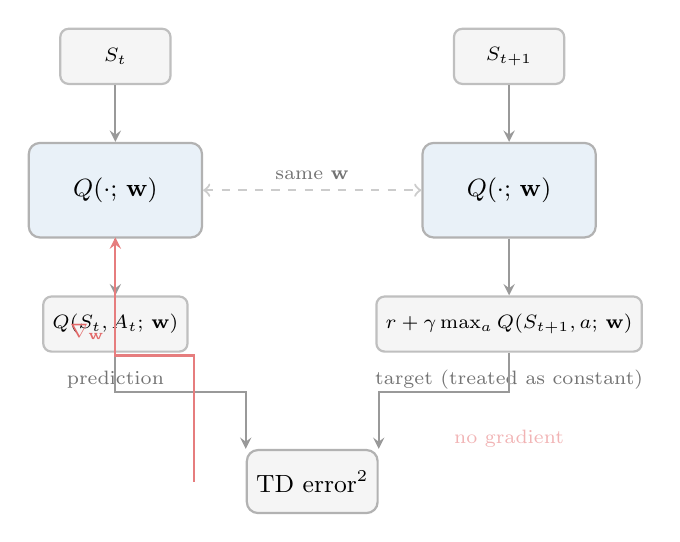
\begin{tikzpicture}[
    net/.style={draw=black!30, thick, rounded corners=4pt,
                minimum width=2.2cm, minimum height=1.2cm,
                font=\small, align=center, inner sep=5pt,
                fill=palA!10},
    io/.style={draw=black!25, thick, rounded corners=3pt,
               minimum width=1.4cm, minimum height=0.7cm,
               font=\scriptsize, fill=black!4, align=center},
    lossbox/.style={draw=black!30, thick, rounded corners=4pt,
                    minimum width=1.4cm, minimum height=0.8cm,
                    font=\small, fill=black!4},
    arr/.style={->, thick, >=stealth, black!40},
    garr/.style={->, thick, >=stealth, palB!60},
    nogarr/.style={thick, palB!25, dashed},
    lbl/.style={font=\scriptsize, text=black!55},
]

% Prediction side (left)
\node[io] (s) at (-2.5, 2.2) {$S_t$};
\node[net] (net1) at (-2.5, 0.5) {$Q(\cdot;\, \mathbf{w})$};
\node[io] (pred) at (-2.5, -1.2)
    {$Q(S_t, A_t;\, \mathbf{w})$};
\node[lbl] at (-2.5, -1.9) {prediction};

\draw[arr] (s) -- (net1);
\draw[arr] (net1) -- (pred);

% Target side (right)
\node[io] (sp) at (2.5, 2.2) {$S_{t+1}$};
\node[net] (net2) at (2.5, 0.5) {$Q(\cdot;\, \mathbf{w})$};
\node[io] (targ) at (2.5, -1.2)
    {$r + \gamma \max_a Q(S_{t+1}, a;\, \mathbf{w})$};
\node[lbl] at (2.5, -1.9) {target (treated as constant)};

\draw[arr] (sp) -- (net2);
\draw[arr] (net2) -- (targ);

% "same w" indicator
\draw[thick, black!20, dashed, <->]
    (net1.east) -- (net2.west)
    node[midway, above, lbl] {same $\mathbf{w}$};

% Loss
\node[lossbox] (loss) at (0, -3.2) {TD error$^2$};
\draw[arr] (pred.south) -- ++(0, -0.5) -| (loss.north west);
\draw[arr] (targ.south) -- ++(0, -0.5) -| (loss.north east);

% Gradient arrow (only to prediction side)
\draw[garr] (-1.5, -3.2) -- (-1.5, -1.6) -- (-2.5, -1.6)
    -- (-2.5, -0.1)
    node[lbl, pos=0.2, left, text=palB!70]
    {$\nabla_{\mathbf{w}}$};

% No gradient on target side (crossed out)
\node[font=\scriptsize, text=palB!35] at (2.5, -2.65)
    {no gradient};

\end{tikzpicture}
\caption{Semi-gradient update. The same parameters $\mathbf{w}$
  produce both the prediction and the target, but the gradient flows
  only through the prediction side.}
\label{fig:semi-gradient}
\end{figure}


\smallskip
Function approximation makes Q-learning applicable to problems that
tabular methods cannot touch: the agent can process raw images,
generalize across similar states, and scale to environments with
vast state spaces. But these gains come at a cost. Tabular
Q-learning converges to $q_*$ under standard conditions; with
nonlinear function approximation, no such guarantee exists in
general.

\smallskip
The instability arises from the combination of three elements,
known as the \emph{deadly triad}~\citep{sutton2018reinforcement}.
First, \emph{bootstrapping}: the TD target depends on the current
estimates, so errors in the Q-values feed back into the targets
used to train them. Second, \emph{off-policy learning}: the $\max$
operator in the target means the agent updates toward a different
policy (the greedy one) than the one it uses to collect data,
which can amplify estimation errors. Third, \emph{function
approximation} itself: because parameters are shared across states,
a single update changes Q-values for many states simultaneously,
and these coupled changes can reinforce each other and cause the
estimates to diverge.

\smallskip
Before describing the specific network architecture used in
practice, we need to understand the building blocks it is made from.
